\chapter{研究现状与相关工作}

\section{三维测距技术}
近年来,三维测距技术得到了越来越广泛的应用。
传统的的三维测距技术通常应用在专业的三维扫描设备中,
但今年来越来越多的公司都推出了搭载三维测距技术的产品与项目,
如Microsoft的Kinect\cite{microsoft_kinect}、
Google的Tango\cite{google_tango} Project,Apple的iPhone X\cite{apple_iphoneX}、Intel的RealSense\cite{intel_realsense}等。
\section{三维重建技术}
三维重建一直是学术界和工业界关注的问题,数十年来有很多相关的科研工作。
这些三维重建的方法将距离信息,如无结构化点云\cite{henry2010rgb}\cite{keller2013real}
\cite{whelan2015elasticfusion}、2.5D深度图像\cite{meilland2013unifying}或高度场\cite{gallup20103d},
转化为基于占据栅格(occupancy grids)\cite{elfes1987sensor}
或隐式曲面(implicit surfaces)的体素表达\cite{curless1996volumetric}。
在很多三维重建工作中,其默认的体素表达是TSDFs(Truncated Signed Distance Felds,
删节有向距离场)\cite{fioraio2015large}\cite{fuhrmann2014floating}。
这些基于TSDF的方法可以建立连续的曲面,系统性的处理噪声,
不需要记录显式的拓扑信息并且能够有效的做增量式的修改。
在这些方法中最有名的就是KinectFusion\cite{izadi2011kinectfusion}\cite{newcombe2011kinectfusion},
它实现了实时的相机跟踪和体素融合。

要利用相机重建三维信息,需要获得两个位置信息:物体表面和相机的相对位置以及相机在世界坐标系中的位姿。
物体和相机的相对位置可通过三维测距技术实现,相机位姿的确定则需要通过相机在每一帧中的位姿实现。
三维测距的相关工作以及在上一节介绍了,
而相机的位姿通常是基于ICP(Iterative Closest Point,迭代最近点)算法
\cite{besl1992method}及其变种实现。
这些方法会计算相邻两帧之间的相机发生的刚体变换,并将其叠加到上一帧的相机位姿上,
增量的计算相机当前的位姿。
在实际的工作中,这样的相机跟踪方法往往鲁棒性不佳,容易引入累计误差。
有很多研究这就会借助RGB图像提升每帧之间的跟踪结果\cite{whelan2013robust}
或者利用全局的位姿估计校正来提升位姿的精度。
常见的全局位姿优化方法有位姿图优化(pose graph optimization)\cite{steinbrucker2013large},
闭环检测(loop closure detection)\cite{whelan2013deformation},
增量式的BA(incremental bundle adjustement)\cite{fioraio2015large}
以及利用关键点进行或图片对相机进行重定位等。
\begin{figure}[h]
    \centering
    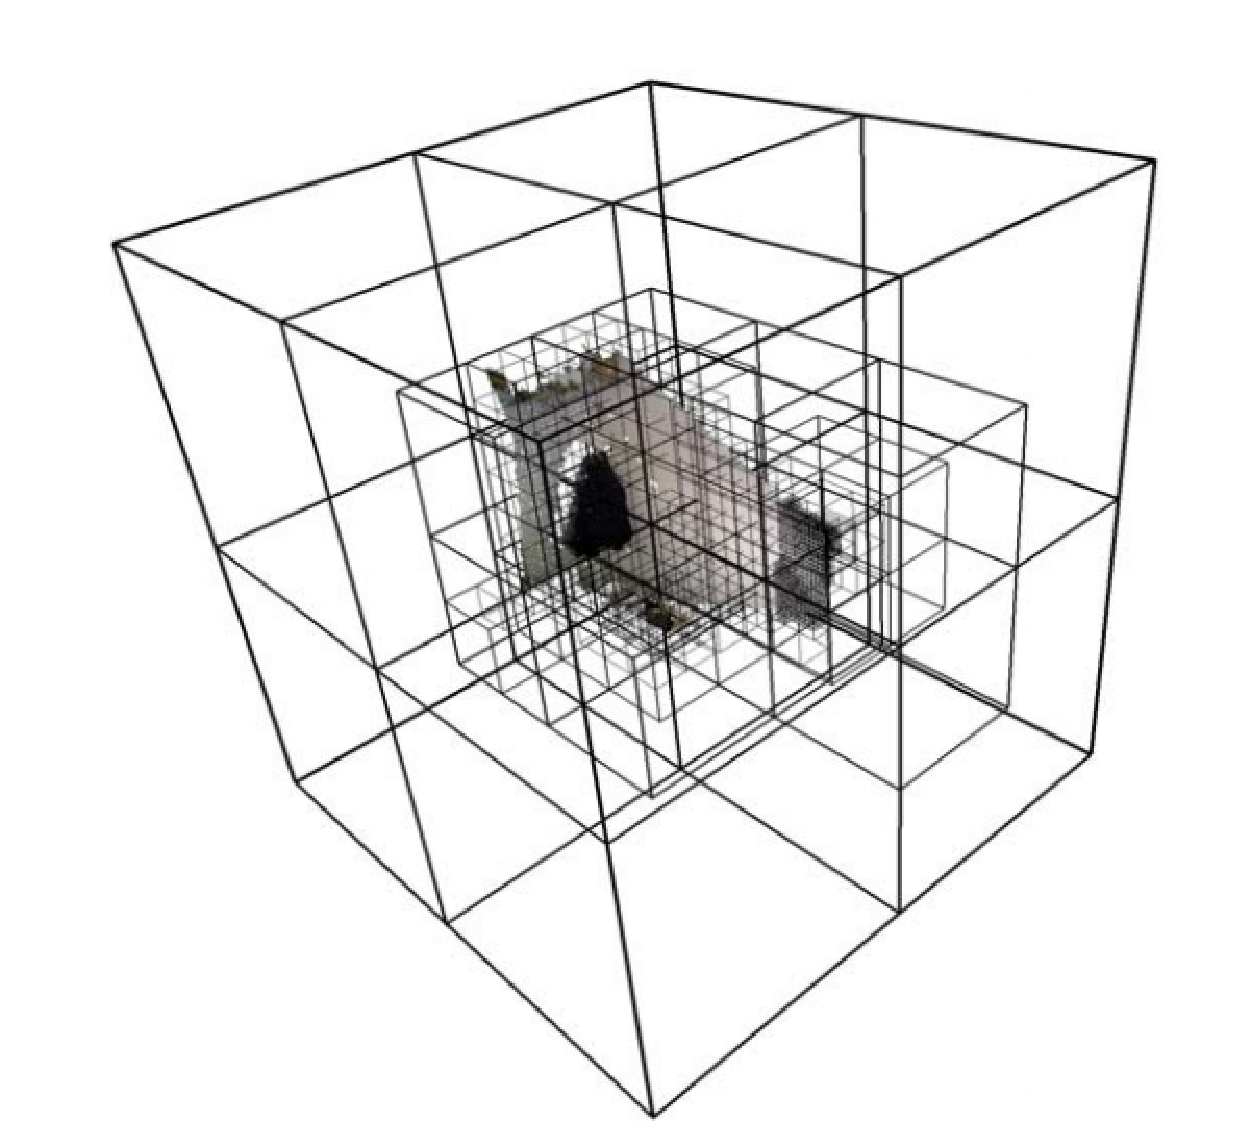
\includegraphics[width = 0.6\textwidth]{./Pictures/octree.eps}
    \caption{八叉树结构}
    \label{octree}
\end{figure}

很多重建算法为了达到实时的性能,都引入了GPU并行实现。
例如KinectFusion\cite{izadi2011kinectfusion}就用GPU实现了将深度图片信息并行的融合到统一化网格的算法。
但体素信息的存储会占用大量的显存,显存大小也就成了场景分辨率的最大瓶颈。
为了突破显存对场景分辨率的限制,有的工作会将不在视野内的体素从显存中换出\cite{roth2012moving}。
Steinbrucker在2013年的工作\cite{steinbrucker2013large}采用了多尺度的八叉树(octree)数据结构
和稠密图对齐实现了大尺度室内场景的重构。
分层空间数据结构和流算法也被利用以将KinectFusion扩展到更大的场景中\cite{chen2013scalable}。
此外,还有相关的工作\cite{niessner2013real}采用体素哈希(voxel hashing)来减少分层数据结构的开销。





\section{三维模型形变技术}
三维模型的形变一直是图形学届所关注的研究课题。
形状建模的早期工作主要聚焦在模型的空间形变,
Barr的工作\cite{barr1984global}就提供了全局的空间重映射。
FFD(Free-form deformation,自由形变)\cite{sederberg1986free}用三维晶格将空间形变参数化,
提供了一个高效的对复杂形状施加粗略形变的方法。
但要得到高质量的形变效果,需要更多细节的控制点\cite{coquillart1990extended},
也会引入更多的手工操作。
常见的网格模型修改工具允许用户移动少量顶点让模型发生形变,同时要保留模型的细节和平滑。
细分和多分辨率技术将网格细节编码为顶点的在拓扑上的
偏移\cite{zorin1997interactive}\cite{kobbelt2000multiresolution}
或者几何上更为简单的基网格\cite{kobbelt1998interactive},
从而在不同的尺度下达到细节保留的目的。
% \begin{figure}[h]
%     \centering
%     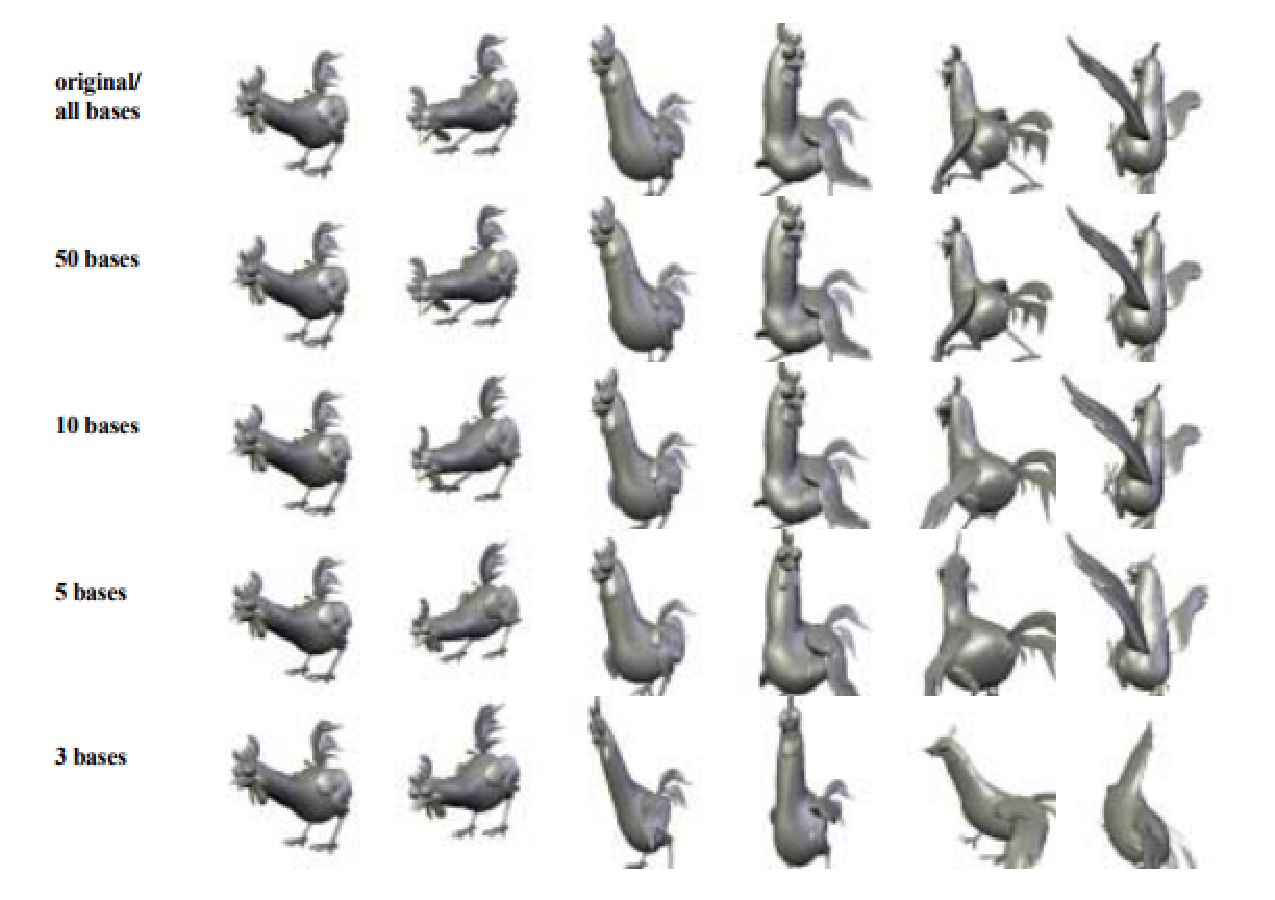
\includegraphics[width=0.95\textwidth]{./Pictures/PCA.eps}
%     \caption{基于PCA的网格动画表示}
%     \label{pca}
% \end{figure}

另一些修改网格的模型的方法则采用了拉普拉斯坐标或金字塔坐标等本征表达。
在这些方法中,每个顶点的位置是由它和相邻节点的关系编码的,
所以局部的改动可以通过本征表达在网格重建的过程中传播的周围的节点。
Yu和Zhou的工作\cite{yu2004mesh}求解了离散在整个网格上的泊松方程。
Sumner提出了形变梯度(deformation-gradient)\cite{sumner2004deformation}来描述形变。
形变梯度描述了三角形网格模型中每一个三角面片相对于参考模型(reference mesh)中对应面片的仿射变换。
Sumner后来提出的Mesh-Based IK\cite{sumner2005mesh}也采用了这种描述形变的方式构建形变子空间,
本文构建子空间采用的也是这一方法。

在三维动画领域,有很多工作致力于基于网格动画序列或集合的压缩表示。
Alexa和Muller\cite{alexa2000representing}用PCA
(Principal Component Analysis,主成分分析)对动画序列。
该方法用一个显现的网格子空间近似表达了网格动画的集合。
相似的,Hauser、Shen和 Brien\cite{hauser2003interactive}
用对弹性方程的模态分析推断所有线性弹性材料的结构共性,
通过对质量和刚度矩阵的特征值分析提取出一组基向量。
该方法易于理解和且实现较为简单但其固有的线性结构导致其不适合描述一些非线性的形变。
比如对于旋转的线性插值会导致网格模型变小。
而且PCA虽然能够很好对已有的网格模型进行压缩,
却不适合构建在主成分所构建的子空间之外的形变。
一些混合式的方法试图解决这一问题,
在某些特殊情况下用骨骼形变描述非线性形变和线性插值相结合\cite{lewis2000pose}。
本文所采用的模型才用了线性插值与非线性插值相结合的方式构建子空间,
对于仿射变换中旋转的部分在李代数上进行插值,对于其他部分则采用线性插值。

\section{形变捕捉技术}
随着深度相机,如Kinect\cite{microsoft_kinect}的普及,产生了很多的静态三维重建的相关工作,
如KinectFusion\cite{newcombe2011kinectfusion}。
在这些研究的基础上,很多研究者希望更进一步,利用深度相机实现动态场景的捕捉。
很多动态场景捕捉的相关工作都关注在人体特定部分的形变捕捉。
这些人体的部位往往具有特殊的形状和既定的运动模式,
这些运动模式可以是通过观察总结的也可以是认为规定的。
有很多高精度高效率的的工作聚焦于人脸\cite{cao20133d}\cite{li2013realtime}、
手\cite{oikonomidis2011efficient}\cite{qian2014realtime}、
身体\cite{taylor2012vitruvian}或铰接件\cite{schmidt2014dart}\cite{ye2014real}的形变。
% \begin{figure}[h]
%     \centering
%     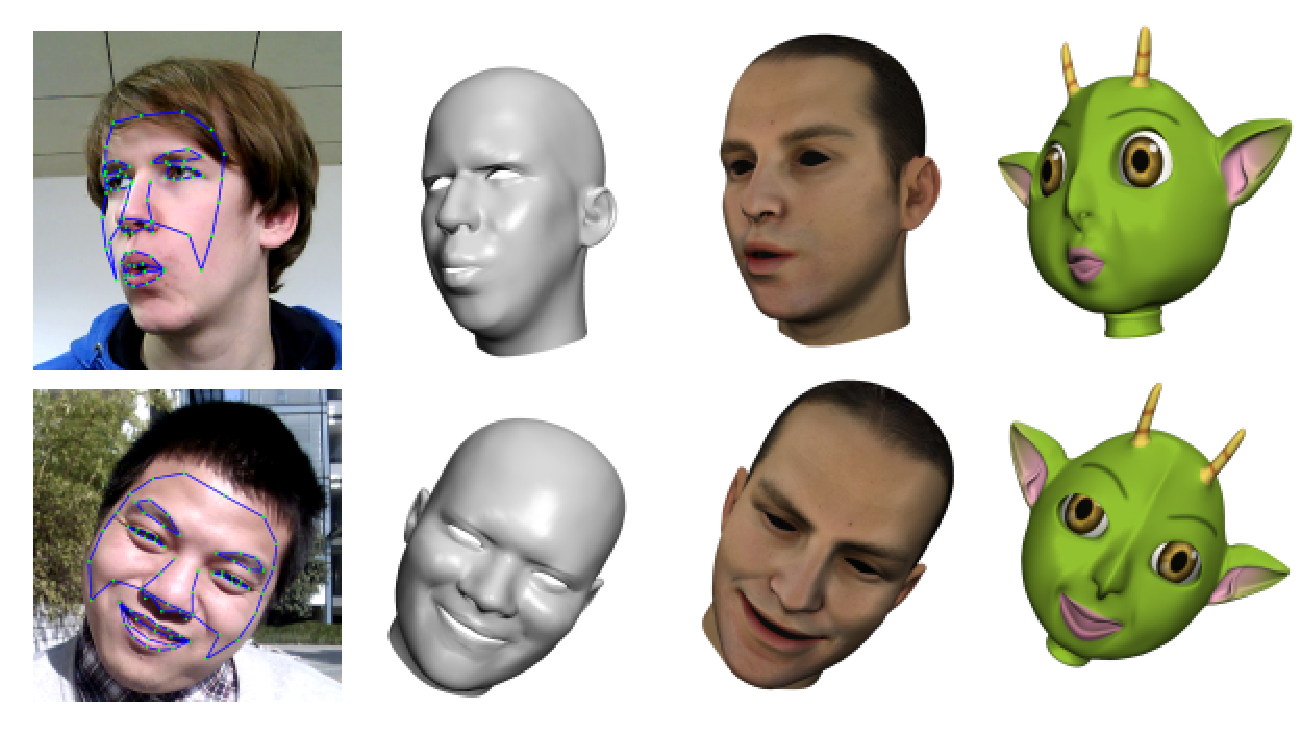
\includegraphics[width = 0.7\textwidth]{./Pictures/facial_animation.eps}
%     \caption{Cao的实时人脸动画捕捉系统}
%     \label{facial_animation}
% \end{figure}
\begin{figure}[h]
    \centering
    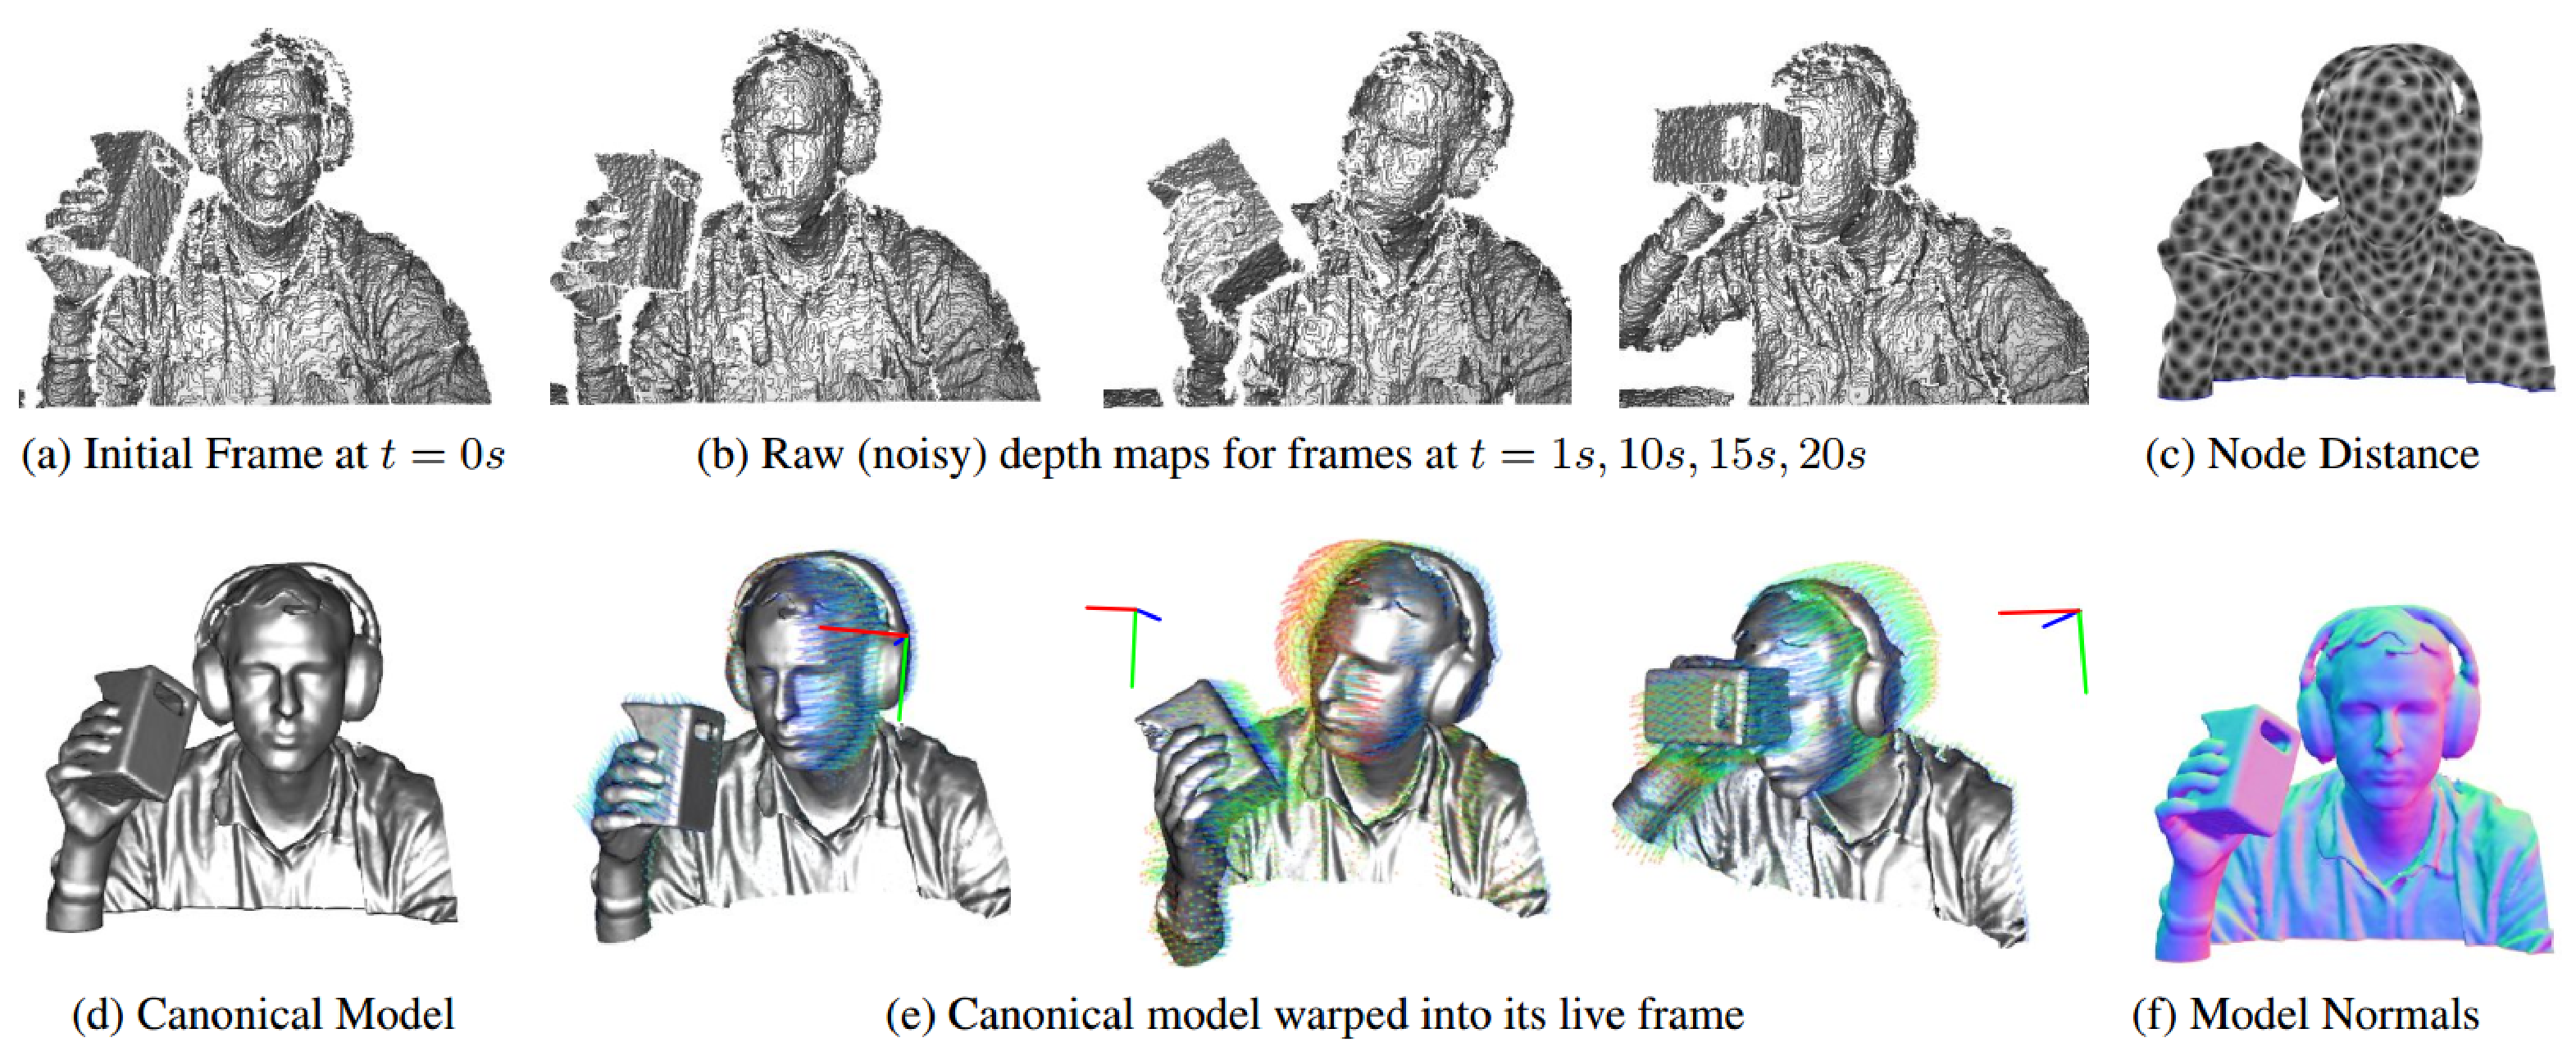
\includegraphics[width = \textwidth]{./Pictures/dynamic_fusion.eps}
    \caption{DynamicFusion——一个实时非刚体SLAM系统}
    \label{dynamic_fusion}
\end{figure}

此外,也有很多研究工作直接捕捉更为通用的网格模型的形变。
Li的工作\cite{li2009robust}通过扫描获取物体模型,
并用一个低分辨率的模型作为先验的形变模板来追踪物体大致的形变,
并通过非刚体重建获得高频的几何细节。
后来,Zollh{\"o}fer\cite{zollhofer2014real}的工作使用了类似的技术,借助GPU加速,
给出了一个高效的实时形变捕捉系统。
在这个系统实时的维护了一个高分辨率的刚体模型,作为非刚体捕捉的先验,以提高形变捕捉的效率。
受到了这些工作的启发,
DynamicFusion\cite{newcombe2015dynamicfusion}给出了一个能够捕捉形变并重建非刚体场景的SLAM系统。
与章节\ref{reconstruction}中所描述的三维重建系统类似,
DynamicFusion维护着一个基于TSDF的静态模型(Canonical Model)。
此外,该工作还维护了一个描述模型形变的非刚体形变场(Non-rigid Warp Field),
用以描述了模型的形变,如图\ref{dynamic_fusion}。
本文的形变捕捉系统主要参考的就是该工作的形变捕捉框架。


\section{本章小结}
本章主要介绍了深度相机、三维重建及三维模型形变的相关工作。
首先阐述了深度相机的概念及其广泛应用,并介绍了目前主流的三维测距技术,
了解了深度相机的工作原理,从而对本文所采用的输入设备有了更深入的理解。
然后介绍了基于扫描设备的三维重建技术,了解了如何将现实世界中的物体扫描为三维模型。
随后分别从模型修改和形变捕捉两个角度介绍了前人在获得静态三维模型之后,
在模型的形变上作出的工作。

